\chapter{Storing Facts in Tries} \label{chap:tries}
\index{tries}

\index{indexing!trie-based}
XSB offers a mechanism by which large numbers of facts can be directly
stored and manipulated in {\em tries}, which can either be private to
a thread or shared among threads.  The mechanism described in this
chapter is in some ways similar to trie-indexed asserted code as
described in Section~\ref{sec:assert}, but allows creation of tries
that are shared between threads, and of associative tries that support
efficient memory management~\footnote{For nearly all purposes, the
  predicates in this chapter replace the low-level API for interned
  tries in previous versions, which included {\tt trie\_intern}, {\tt
    trie\_unintern}, {\tt trie\_interned} etc.  However that API
  continues to be supported for low-level systems programming.}.

When stored in a trie, facts are compiled into trie-instructions
similar to those used for XSB's tables.  For instance set of facts
\begin{center}
\{ {\tt rt(a,f(a,b),a), rt(a,f(a,X),Y), rt(b,V,d)} \} 
\end{center}
would be stored in a trie as shown in Figure~\ref{fig:trie}, where
each node corresponds to an instruction in XSB's virtual machine.
\begin{figure}[htbp] \label{fig:trie}
\centering
\begin{tabular}{c}
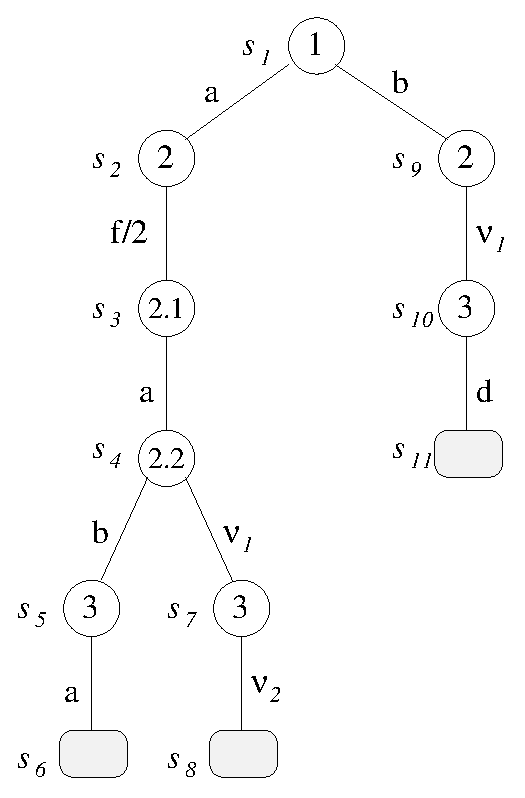
\includegraphics[width=0.3\textwidth]{trie}
%%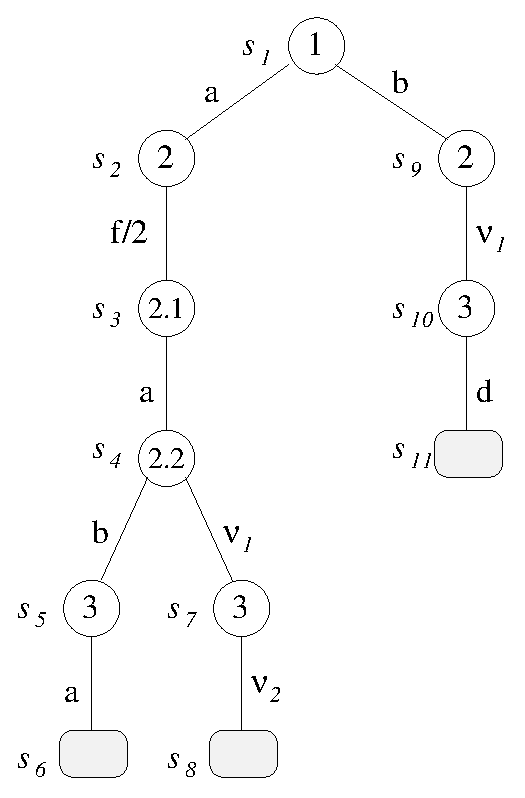
\epsfig{file=trie,height=.3\textheight}
\end{tabular}
\caption{Terms Stored as a Trie}
\end{figure} 
Using a trie for storage has the advantage that discrimination can be
made on a position anywhere in a fact, and directly inserting into or
deleting from a trie is 4-5x faster than with standard dynamic code.
In addition, in trie-dynamic code, there is no distinction between the
index and the code itself, so for many sets of facts trie storage can
use much less space than standard dynamic code.  For instance,
Figure~\ref{fig:trie} shows how the prefix {\tt rt(a,f(a,...} is
shared for the first two facts.  However, trie storage comes with
tradeoffs: first, only facts can be stored in a trie; second, unlike
standard dynamic code, no ordering is preserved among the facts; and
third, duplicate facts are not supported.

In \version{} of XSB, tries that store facts may have the following
forms:
%
\bi
\item {\em Private, general} tries allow arbitrary terms to be
  inserted in a trie.  These tries are thread-private so that
  inserting a term in a trie $Tr$ in one thread will not be visible to
  another thread.  Although such tries are general, they have
  limitations in memory reclamation in \version{} of XSB.  If a term
  is deleted from $Tr$, memory will be reclaimed if it is safe to do
  so at the time of deletion~\footnote{That is, if no choice points
    are around that may cause backtracking into $Tr$.}; otherwise the
  space will not be reclaimed until all terms in $Tr$ are removed by
  truncating $Tr$ or until the thread exits.

\item {\em Private, associative} Associative tries are more restricted
  than general tries: an associative trie combines a {\em key} which
  can be any ground term, with a {\em value} which can be any term.
  Memory for deleted key-value pairs in an associative trie is always
  immediately reclaimed, and insert or delete operations can be faster
  for an associative trie than for a general trie.  These tries are
  private to a thread, and in addition to reclaiming memory when a
  term is deleted, memory is reclaimed when the trie is truncated or
  dropped, and when the thread exits.

\item {\em Shared, associative} tries are associative tries that are
  shared among threads.  Memory for deleted key-value pairs is always
  immediately reclaimed, and when the trie is truncated or dropped.
  \ei

\section{Examples of Using Tries}

A handle for a trie can be obtained using the {\tt trie\_create/2}
predicate.  Terms can then be inserted into or deleted from that trie,
and terms can be unified with information in the trie, as shown in the
following example:

\begin{example} \rm
First, we create a private general trie: 
{\small
\begin{verbatim}
| ?- trie_create(X,[type(prge)]).
X = 1

yes
\end{verbatim}
}
%
Next, we insert some terms into the trie
{\small
\begin{verbatim}
| ?- trie_insert(1,f(a,b)), trie_insert(1,[a,dog,walks]).

yes
\end{verbatim}
}
Now we can make arbitrary queries against the trie
{\small
\begin{verbatim}
| ?- trie_unify(1,X).

X = [a,dog,walks];

X = f(a,b);

no
\end{verbatim}
}
\noindent
Above, a general query was made, but the query could have been any
Prolog term.  Now we delete a term, and see what's left.
{\small
\begin{verbatim}
| ?- trie_delete(1,f(X,B)).

X = a
B = b

yes
| ?- trie_unify(1,X).

X = [a,dog,walks];

no
\end{verbatim}
}
\end{example}

The behavior of general tries can be constrasted with that of
associative tries as seen in the next example.
\begin{example} \rm
Now we start by creating a shared associative trie, with abbreviation
{\tt shas} using the multi-threaded engine
{\small
\begin{verbatim}
| ?- trie_create(X,[type(shas),alias(foo)]).
X = 1048577

yes
\end{verbatim}
}  \noindent
%
This time we used an alias so now we can use {\tt foo} to refer to
insert a couple of key-value pairs into the trie (we could also use
the trie handle itself) 
{\small
\begin{verbatim}
| ?- trie_insert(foo,pair(sentence(1),[a,dog,walks])), 
     trie_insert(foo,pair(sentence(2),[a,man,snores])).

yes
\end{verbatim}
} \noindent
However, inserting a general term into an associative trie throws an
error
{\small
\begin{verbatim}
| ?- trie_insert(foo,f(a,b)).
++Error[XSB/Runtime/P]: [Domain (f(a,b) not in domain pair/2)]  
in arg 2 of predicate trie_insert/2 
(Inserted term must be key-value pair in trie 1048577)
\end{verbatim}
}  \noindent
Finally, in an associative trie, if we insert a value for a key that
is already in the trie, it will {\em update} the value for that key.
{\small
\begin{verbatim}
| ?- trie_insert(foo,pair(sentence(1),[a,dog,snoress])).

yes
| ?- trie_unify(foo,pair(sentence(1),X)).
X = [a,dog,snores]

yes
\end{verbatim}
}

\end{example}

\section{Predicates for Tries} 
%
The following subsections describe predicates for inserting terms into
a trie, deleting terms from a trie, and unifying a term with terms in
a trie, predicates for creating, dropping, and truncating tries, as
well as predicates for bulk insertes into and deletes from a trie.
These predicates can apply to any type of trie, and perform full error
checking on their call arguments.  As such, they are safer and more
general than the lower-level trie predicates described in Chapter 1 of
Volume 2 of this manual.  Use of the predicates described here is
recommended for applications unless the need for speed is paramount.

\begin{description}
%
\index{aliases!tries}
\ourmoditem{trie\_create(-TrieId,+OptionList)}{trie\_create/2}{intern}
%
{\tt OptionList} allows optional parameters in the configuration of a
trie to indicate its type and whether an alias should be used.  In the
present version, {\tt OptionList} may contain the following terms
\bi
\item {\tt type(Type)} where {\tt Type} can be one of
\bi
\item {\tt prge} (private, general) maintains information that is
  accessable only to the calling thread.  No other restrictions are
  made for accessing information in a private trie.  In the
  single-threaded engine, tries are private by default.

\item {\tt pras} (private, associative) creates a private trie that
  maintains key-value pairs in a manner similar to an associative
  array, using the term {\tt pair(Key,Value)}.  Each key must be ground,
  and there may be only one value per key.

\item {\tt shas} (shared associative) creates a shared trie that
  maintains key-value pairs in a manner similar to an associative
  array, using the term {\tt pair(Key,Value)}.  Each key must be
  ground, and there may be only one value per key.  This option is
  available only in the multi-threaded engine

%\item {\tt shared(full)} Maintains information that is accessable to
%  all threads, with no restrictions on its access.  In the
%  single-threaded engine, there is no distinction between private and
%  shared tries.
\ei
\item {\tt alias(Alias)}: Allow trie {\tt TrieId} to be referred to
  via {\tt Alias} in all standard trie predicates.  {\tt Alias}
  remains active for {\tt TrieId} until it is dropped.
%
\item {\tt incremental}: Allows tables that depend on trie {\tt
  TrieId} to be automatically updated as information in {\tt TrieId}
  changes (cf. Section~\ref{sec:incr-update-tries}).
%
\item {\tt nonincremental}: Specifies that tables that depend on trie
  {\tt TrieId} should not be automatically updated as information in
  {\tt TrieId} changes (cf. Section~\ref{sec:incr-update-tries}).
\end{itemize}
%
{\bf Error Cases}
\bi
\item 	{\tt TrieId} is not a variable
\bi
\item 	{\tt type\_error(variable,TrieId)}
\ei
\item 	{\tt OptionList} is a partial list or contains an option that is a variable
\bi
\item 	{\tt instantiation\_error}
\ei
\item 	{\tt OptionList} is neither a list nor a partial list
\bi
\item 	{\tt type\_error(list,OptionsList)}
\ei
\item 	{\tt OptionList} contains an option, {\tt Option} not described above
\bi
\item 	{\tt domain\_error(trie\_option,Option)}
\ei
\item An element of {\tt OptionsList} is alias(A) and A is already
  associated with an existing thread, queue, mutex or stream 
\bi
\item {\tt permission\_error(create,alias, A)}
\ei
\item An element of {\tt OptionsList} is alias(A) and A its not an atom
\bi
\item {\tt type\_error(atom,A)}
\ei
\ei
\index{tabling!incremental}

\index{terms!cyclic}
\ourmoditem{trie\_insert(+TrieIdOrAlias,Term)}{trie\_insert/2}{intern}
%
Inserts {\tt Term} into the trie denoted by {\tt TrieIdOrAlias}.  If
{\tt TrieIdOrAlias} denotes an associative trie, {\tt Term} must be of
the form {\tt pair(Key,Value)} where {\tt Key} is ground.  If {\tt
  TrieIdOrAlias} is a general trie and already contains {\tt Term},
the predicate fails (as the same term cannot be inserted multiple
times in the same trie).  Similarly, if {\tt TrieIdOrAlias} is an
associative trie and already contains a value for {\tt Key} the
predicate fails.

Insertion of tries can be controlled by the flags {\tt
  max\_answer\_term\_depth}, {\tt max\_answer\_list\_depth}, {\tt
  max\_answer\_term\_action}, and {\tt max\_answer\_list\_action},
which are also used to control additions of answers to tables.  Using
these flags, if a term to be inserted is cyclic and exceeds a stated
depth, trie insertion may either fail or throw an error depending on
the associated action: see pg. \pageref{prolog-flags}.

{\bf Error Cases}
\bi
\item 	{\tt TrieIdOrAlias} is a variable
\bi
\item 	{\tt instantiation\_error}.
\ei
\item 	{\tt TrieIdOrAlias} is not a trie id or alias
\bi
\item 	{\tt domain\_error(trie\_id\_or\_alias,TrieIdOrAlias)}
\ei
\item 	{\tt TrieIdOrAlias} denotes an associative array, and {\tt Term} 
  does not unify with {\tt pair(\_,\_)} 
\bi
\item 	{\tt domain\_error(pair/2,Term)}
\ei
\item 	{\tt TrieIdOrAlias} denotes an associative array, 
  {\tt Term = pair(Key,Value)} but {\tt Key} is not ground 
\bi
\item 	{\tt misc\_error}
\ei
\item {\tt Key} or {\tt Value} is a cyclic term, or exceeds the depth 
\bi
\item 	{\tt misc\_error}
\ei
\ei
%

\ourmoditem{trie\_unify(+TrieIdOrAlias,Term)}{trie\_unify/2}{intern}
%
Unifies {\tt Term} with a term in the trie denoted by {\tt
  TrieIdOrAlias}.  If {\tt TrieIdOrAlias} denotes a general trie,
successive unifications will succeed upon backtracking.  If {\tt
  TrieIdOrAlias} denotes an associative trie, {\tt Term} must be of
the form {\tt pair(Key,Value)} where {\tt Key} is ground.

{\bf Error Cases}
\bi
\item 	{\tt TrieIdOrAlias} is a variable
\bi
\item 	{\tt instantiation\_error}.
\ei
\item 	{\tt TrieIdOrAlias} is not a trie id or alias
\bi
\item 	{\tt domain\_error(trie\_id\_or\_alias,TrieIdOrAlias)}
\ei
\item 	{\tt TrieIdOrAlias} denotes an associative array, and {\tt Term} 
  does not unify with {\tt pair(\_,\_)} 
\bi
\item 	{\tt domain\_error(pair/2,Term)}
\ei
\item {\tt TrieIdOrAlias} denotes an associative array, 
  {\tt Term = pair(Key,Value)} but {\tt Key} is not ground 
\bi
\item 	{\tt misc\_error}
\ei
\ei

\ourmoditem{trie\_delete(+TrieIdOrAlias,Term)}{trie\_delete/2}{intern}
%
Deletes a term unifying with {\tt Term} from the trie denoted by {\tt
  TrieIdOrAlias}.  {\tt TrieIdOrAlias} denotes a general trie, all
such terms can be deleted upon backtracking.  If {\tt TrieIdOrAlias}
denotes an associative trie, {\tt Term} must be of the form {\tt
  pair(Key,Value)} where {\tt Key} is ground.  In either case, if {\tt
  TrieIdOrAlias} does not contain a term unifying with {\tt Term} the
preicate fails.

{\bf Error Cases}
\bi
\item 	{\tt TrieIdOrAlias} is a variable
\bi
\item 	{\tt instantiation\_error}.
\ei
\item 	{\tt TrieIdOrAlias} is not a trie id or alias
\bi
\item 	{\tt domain\_error(trie\_id\_or\_alias,TrieIdOrAlias)}
\ei
\item 	{\tt TrieIdOrAlias} denotes an associative array, and {\tt Term} 
  does not unify with {\tt pair(\_,\_)} 
\bi
\item 	{\tt domain\_error(pair/2,Term)}
\ei
\item {\tt TrieIdOrAlias} denotes an associative array, 
  {\tt Term = pair(Key,Value)} but {\tt Key} is not ground 
\bi
\item 	{\tt misc\_error}
\ei
\ei
%
\ourmoditem{trie\_truncate(+TrieIdOrAlias)}{trie\_truncate/1}{intern}
%
Removes all terms from {\tt TrieIdOrAlias}, but does not change any of
its properties (e.g. the type of the trie or its aliases).  

{\bf Error Cases}
\bi
\item 	{\tt TrieIdOrAlias} is a variable
\bi
\item 	{\tt instantiation\_error}.
\ei
\item 	{\tt TrieIdOrAlias} is not a trie id or alias
\bi
\item 	{\tt domain\_error(trie\_id\_or\_alias,TrieIdOrAlias)}
\ei
\ei

\ourmoditem{trie\_drop(+TrieIdOrAlias)}{trie\_drop/1}{intern}
%
Drops {\tt TrieIdOrAlias}.  {\tt trie\_drop/1} not only removes all
terms from {\tt TrieIdOrAlias}, but also removes information about its
type and any aliases the trie may have.

{\bf Error Cases}
\bi
\item 	{\tt TrieIdOrAlias} is a variable
\bi
\item 	{\tt instantiation\_error}.
\ei
\item 	{\tt TrieIdOrAlias} is not a trie id or alias
\bi
\item 	{\tt domain\_error(trie\_id\_or\_alias,TrieIdOrAlias)}
\ei
\ei

\ourmoditem{trie\_bulk\_insert(+TrieIdOrAlias,+Generator)}{trie\_bulk\_insert/2}{intern}
% 
Used to insert multiple terms into the trie denoted by {\tt
  TrieIdOrAlias}.  {\tt Generator} must be a callable term.  Upon
backtracking through {\tt Generator} its first argument should
successively be instantiated to the terms to be interned in {\tt
  TrieIdOrAlias}.  When inserting many terms into a general trie, {\tt
  trie\_bulk\_insert/2} is faster than repeated calls to {\tt
  trie\_insert/2} as it does not need to make multiple checks that the
choice point stack is free of failure continuations that point into
the {\tt TrieIdOrAlias} trie.  For associative tries, {\tt
  trie\_bulk\_insert/2} can also be faster as it needs to perform
fewer error checks on the arguments of the insert.

\begin{example} \rm
Given the predicate 
\begin{verbatim}
bulk_create(p(One,Two,Three),N):- 
     for(One,1,N),
     for(Two,1,N),
     for(Three,1,N).
\end{verbatim}
and a general trie {\tt Trie}, the goal 
\begin{center}
   {\tt ?- trie\_bulk\_insert(Trie,bulk\_create(\_Term,N))} 
\end{center}
will add $N^3$ terms to {\tt Trie}.
\end{example}

{\bf Error Cases}
\bi
\item 	{\tt TrieIdOrAlias} is a variable
\bi
\item 	{\tt instantiation\_error}.
\ei
\item 	{\tt TrieIdOrAlias} is not a trie id or alias
\bi
\item 	{\tt domain\_error(trie\_id\_or\_alias,TrieIdOrAlias)}
\ei
\item   {\tt Generator} is not a compound term
\bi
\item   {\tt type\_error(compound,Generator)}
\ei
\item 	{\tt TrieIdOrAlias} denotes an associative array, and {\tt Generator} 
  does not unify with {\tt pair(\_,\_)} 
\bi
\item 	{\tt domain\_error(pair/2,Term)}
\ei
\item {\tt TrieIdOrAlias} denotes an associative array, and {\tt
  Generator} succeeds with a term that unifies with {\tt
  pair(Key,Value)} and {\tt Key} is not ground 
\bi
\item 	{\tt misc\_error}
\ei
\item {\tt Key} or {\tt Value} is a cyclic term
\bi
\item 	{\tt misc\_error}
\ei
\ei

\index{terms!cyclic}
\ourmoditem{trie\_bulk\_delete(+TrieIdOrAlias,Term)}{trie\_bulk\_delete/2}{intern}
% 
Deletes all terms that unify with {\tt Term} from {\tt TrieIdOrAlias}.
If {\tt TrieIdOrAlias} denotes an associative trie, the key of the key
value pair need {\em not} be ground.

\begin{example}\label{ex:bulk-delete} \rm
For the trie in the previous example, the goal 
\begin{center}
{\tt ?-  trie\_bulk\_delete(Trie,p(1,\_,\_))} 
\end{center}
will delete the $N^2$ terms that unify with {\tt p(1,\_,\_)} from {\tt TrieIdOrAlias}.
\end{example}

{\bf Error Cases}
\bi
\item 	{\tt TrieIdOrAlias} is a variable
\bi
\item 	{\tt instantiation\_error}.
\ei
\item 	{\tt TrieIdOrAlias} is not a trie id or alias
\bi
\item 	{\tt domain\_error(trie\_id\_or\_alias,TrieIdOrAlias)}
\ei
\ei

\ourmoditem{trie\_bulk\_unify(+TrieIdOrAlias,\#Term,-List)}{trie\_bulk\_unify/3}{intern}
% 
Returns in {\tt List} all terms in {\tt TrieIdOrAlias} that unify with
{\tt Term}.  If {\tt TrieIdOrAlias} denotes an associative trie, the
key of the key value pair need {\em not} be ground.

This predicate is useful for two reasons.  First, it provides a safe
way to backtrack through an associative trie while maintaining the
memory management and concurrency properties of associative tries.
Second, it enforces read consistency for {\tt TrieIdOrAlias},
regardless of whether the trie is private or shared, general or
associative.

\begin{example} \rm
Continuing from Example~\ref{ex:bulk-delete} the goal
\begin{center}
{\tt ?-  trie\_bulk\_unify(Trie,X),List} 
\end{center}
will return the the $N^3 - N^2$ terms still in {\tt TrieIdOrAlias}.
\end{example}

{\bf Error Cases}
\bi
\item 	{\tt TrieIdOrAlias} is a variable
\bi
\item 	{\tt instantiation\_error}.
\ei
\item 	{\tt TrieIdOrAlias} is not a trie id or alias
\bi
\item 	{\tt domain\_error(trie\_id\_or\_alias,TrieIdOrAlias)}
\ei
\item 	{\tt List} is not a variable
\bi
\item 	{\tt type\_error(variable,List)}.
\ei
\ei

\ourmoditem{trie\_property(?TrieOrAlias,?Property)}{trie\_property/2}{intern}
%
If {\tt TrieOrAlias} is instantiated, unifies {\tt Property} with
current properties of the trie; if {\tt TrieOrAlias} is a variable,
backtracks through all the current tries whose properties unify with
{\tt Property}.  In the MT engine, {\tt thread\_property/2} accesses
only tries private to the calling thread and shared tries; however
note that there is no guarantee that that the information returned
about shared tries will be valid, due to concurrency
issues~\footnote{{\tt trie\_property/2} is not yet implemented for
  shared tries.}.

Currently {\tt Property} can have the form 
\bi
\item {\tt type(Type)}: where {\tt Type} is the type of the trie.
%
\item {\tt alias(Alias)}: if the trie has an alias {\tt Alias}
\ei

{\bf Error Cases}
%
\bi
\item {\tt TrieOrAlias} is neither a variable nor an XSB trie id
  nor an alias
\bi
\item {\tt domain\_error(trie, TrieOrAlias)}
\ei
\item {\tt TrieOrAlias} is not associated with a valid trie
\bi
\item {\tt existence\_error(trie, TrieOrAlias)}
\ei
\ei

%\ouritem{trie\_property(+TrieIdOrAlias,Property)}
%\index{\texttt{trie\_property/2}}
%
\end{description}

